%\documentclass[a4paper]{article}
%\usepackage{graphicx}
%\usepackage{eepic}
%\usepackage{pst-all}
%\usepackage{amsmath, amsthm,amsfonts, stmaryrd}
%%\usepackage[latin1]{inputenc}
%\usepackage[cyr]{aeguill}
%%\usepackage[francais]{babel}
%\usepackage{listings}
%\usepackage{psfrag}
%\usepackage{epsfig}

%%\usepackage{pdftricks}

%%\usepackage{bookman}
%%\usepackage{helvet}
%%\usepackage{newcent}
%%\usepackage{aeguill}

%

%\DeclareMathOperator{\sinc}{sinc}

%
%\renewcommand{\v}{\vec} 
%\renewcommand{\c}{\times} 
%\renewcommand{\o}{\circ}
%\renewcommand{\b}{\mathbf} 

%\newcommand{\w}{\omega} 
%\newcommand{\IM}{\vec{\textrm{Im}}} 
%\newcommand{\RE}{\textrm{Re}} 

%

%%\lstset{language=MATLAB}
%%\lstset{basicstyle=\footnotesize,frame=single}

%%\newenvironment{nom}[nb_arg]{avant}{aprs}

%\newcommand{\projectName}{\emph{hydroMEX3 }} %current project name

%%MATLAB code listings:
%\newcommand{\MATcode}
%{
%	\lstset{language=MATLAB}
%	\lstset{basicstyle=\footnotesize,frame=single,showstringspaces=false}
%}
%%MATLAB code line:
%\newcommand{\MATline}
%{
%	\lstset{language=MATLAB}
%	\lstset{basicstyle=\normalsize,frame=none,showstringspaces=false}
%}
%%C code listings:
%\newcommand{\Ccode}
%{
%	\lstset{language=C}
%	\lstset{basicstyle=\footnotesize,frame=single,showstringspaces=false}
%}
%%C code line:
%\newcommand{\Cline}
%{
%	\lstset{language=C}
%	\lstset{basicstyle=\normalsize,frame=none,showstringspaces=false}
%}

%
%\newcommand{\vbeg}{\left( \begin{array}{c} } 
%\newcommand{\vend}{ \end{array} \right)} 

%\definecolor{cBlue}{rgb}{0.0,0.0,1.0}
%\definecolor{cViol}{rgb}{0.4,0.0,0.6}
%\definecolor{cRed}{rgb}{0.7,0.0,0.3}
%\definecolor{cGreen}{rgb}{0.3,0.5,0.0}
%\definecolor{cGrey}{rgb}{0.2,0.2,0.2}
%\definecolor{cGreyy}{rgb}{0.5,0.5,0.5}
%\definecolor{cBlack}{rgb}{0.0,0.0,0.0}

%\newcommand{\Blue}{\color{cBlue}} 
%\newcommand{\Viol}{\color{cViol}} 
%\newcommand{\Red}{\color{cRed}} 
%\newcommand{\Green}{\color{cGreen}} 
%\newcommand{\Grey}{\color{cGrey}} 
%\newcommand{\Greyy}{\color{cGreyy}} 
%\newcommand{\Black}{\color{cBlack}} 

%
%\begin{document}

%%titre etc...:
%\title{Speed Composition}
%\author{Basile Graf }
%\date{\today}
%\maketitle

%

%

%

%

%\section{}
%\subsubsection{Speed Composition}
%\label{SpeedComposition}




\section{速度组合}
\label{SpeedComposition}


设有三个参考系,分别设计为 $0$, $1$ 和 $2$。参考系 $0$ 是惯性的,参考系 $1$ 是旋转的, 而 $2$ 是机体的固定参考系。\\
同一个向量 $\v{x}$ 可以表示在这些参考系中的任何一个中;当用 $0$表示时,我们将其标记为 $\v{x}^0$,当用 $1$ 表示时,它将标记为 $\v{x}^1$ 和 $\v{x}^2$ 于参考系 $2$ 中。我们还将写 $x^i$ 的四元数 $(0,\v{x}^i)$。\\
此外,还定义了三个四元数: $q_{01}$ 表示参考系 $1$ 相对于参考系 $0$ 的相对姿态, $q_{12}$ 表示参考系 $2$ 相对于参考系 $1$ 的相对姿态,而 $q_{02}$ 表示参考系 $2$ 相对于参考系 $0$的相对姿态。\\


%\begin{figure}
\begin{center}
\psfrag{q01}[l][c][1][0]{$q_{01}$}
\psfrag{q12}[l][c][1][0]{$q_{12}$}
\psfrag{q02}[l][c][1][0]{$q_{02}$}
\psfrag{Ref0}[l][c][1][0]{$0$}
\psfrag{Ref1}[l][c][1][0]{$1$}
\psfrag{Ref2}[l][c][1][0]{$2$}
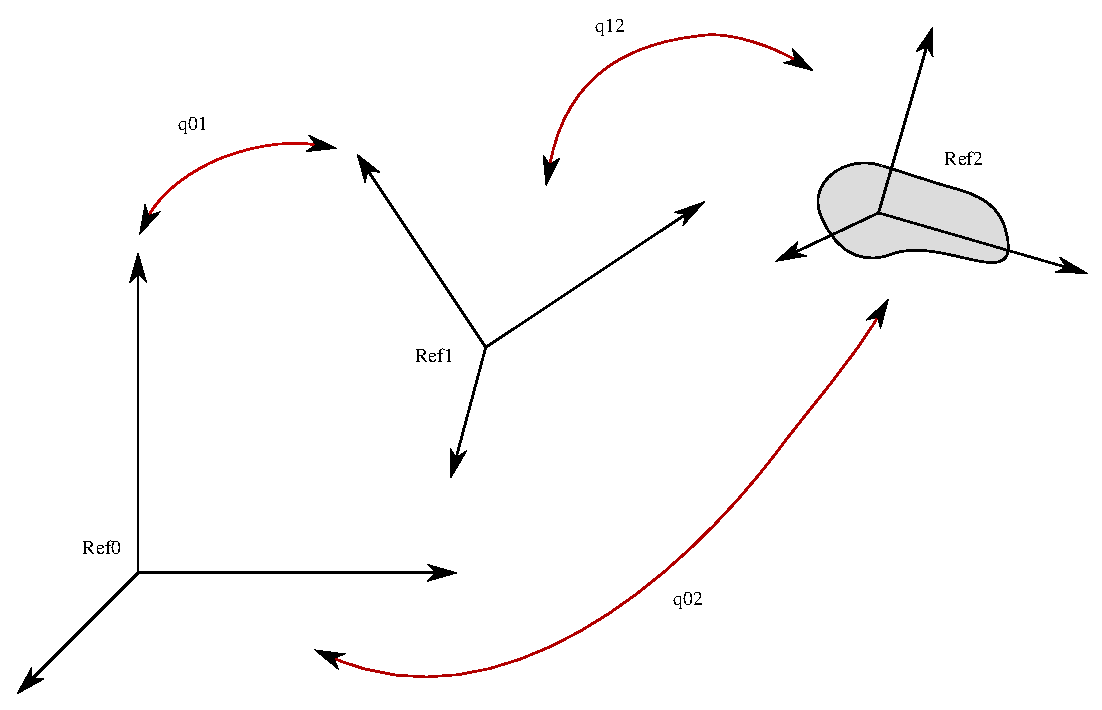
\epsfig{file=figures/SpeedComposition.eps, width=12cm}
\end{center}
%\end{figure}


所以我们可以写为

\begin{equation*}
x^0=q_{01} \o x^1 \o \bar{q}_{01}   \qquad   x^1=q_{12} \o x^2 \o \bar{q}_{12} \qquad    x^0=q_{02} \o x^2 \o \bar{q}_{02}
\end{equation*}

并且替换

\begin{equation*}
x^0=q_{01} \o x^1 \o \bar{q}_{01}  =  q_{01} \o q_{12} \o x^2 \o \bar{q}_{12} \o \bar{q}_{01} 
  =  (q_{01} \o q_{12}) \o x^2 \o (\overline{q_{01} \o q_{12}})
\end{equation*}
  
我们可以确定 $q_{02}$

\begin{equation}
q_{02} = q_{01} \o q_{12}.
\end{equation}

注意 $\omega_{ij}^j = (0,\v{\omega}_{ij}^j)$ 在帧 $j$ 中表示的参考帧 $j$ 相对于帧 $i$ 的旋转速度,并记住 $\omega_{ij}^j = 2\bar{q}_{ij} \o \dot{q}_{ij}$,我们可以写为

\begin{align*}
\omega_{02}^2  &=   2\bar{q}_{02} \o \dot{q}_{02} \\
                              &=   2 (\bar{q}_{12} \o \bar{q}_{01}) \o (\dot{q}_{01} \o q_{12}    +   q_{01} \o \dot{q}_{12}) \\
                              &=   2 \bar{q}_{12} \o \bar{q}_{01} \o \dot{q}_{01} \o q_{12}    +
                                        2 \bar{q}_{12} \o \underbrace{\bar{q}_{01} \o  q_{01}}_{Id} \o \dot{q}_{12} \\
                              &=   \bar{q}_{12} \o \underbrace{(2 \bar{q}_{01} \o \dot{q}_{01})}_{\omega_{01}^1} \o q_{12}    +
                                         \underbrace{2 \bar{q}_{12} \o  \dot{q}_{12}}_{\omega_{12}^2}\\
                              &=  \bar{q}_{12} \o \omega_{01}^1 \o q_{12}    +      \omega_{12}^2 \\
                              &=   \omega_{01}^2   +      \omega_{12}^2.
\end{align*}

也就是说,我们可以添加连续的转速,如果它们表示在同一个参考。\\
在 Cubsat 的情况下, $\v{\omega}_{02}^2$ 是惯性参考模型中以机体坐标表示的卫星的旋转速度 $\v{\omega}'$ ;我们将在这里注意到它 $\v{\omega}'_{Inertial}$ 。另一方面, $\v{\omega}_{12}^2$ 是卫星在非惯性参考模型 (即在轨道参考系中,ORF) 中的旋转速度 $\v{\omega}'$ ;我们会注意到 $\v{\omega}'_{NonInertial}$。 \\
$\v{\omega}_{01}^1$ 是 ORF 中表示的 ORF,即 $\v{\omega}_o$,而 $\v{\omega}_{01}^2$ 是相同的矢量,在机体参考系中变换。这个转换是由非惯性模型 (在上面展开的是 $\bar{q}_{12}$)中的 $R^T$ 执行的。\\
换句话说,我们可以将惯性和非惯性公式(模型)中的 $\v{\omega}'$ 链接在一起

\begin{equation}
\v{\omega}'_{Inertial} = R^T_{NonInertial} \v{\omega}_o + \v{\omega}'_{NonInertial}.
\label{SC_comp}
\end{equation}

这是用来计算非惯性模型动能的速度。




%Bibliographie:
%\begin{thebibliography}{9}

%\bibitem{QFREP}
%	Quaternion, Finite Rotation and Euler Parameters\\
%	Arend L. Schwab \\
%	\emph{http://tam.cornell.edu/\~{}als93/quaternion.pdf}
%	
%\bibitem{Gros}
%	Quaternion based dynamics - Single Turbine Aircraft - Lagrange and Hamiltonian approaches \\
%	S. Gros\\
%	LA, EPFL.
%		
%\bibitem{Gold}
%	Classical Mechanics \\
%	Herbert Goldstein.
%	
%\bibitem{Wells}
%	Lagrangian Dynamics \\
%	Dare A. Wells \\
%	Schaum's Outline Series.
	
	

%	\bibitem{lamport94}
%	  Leslie Lamport,
%	  \emph{\LaTeX: A Document Preparation System}.
%	  Addison Wesley, Massachusetts,
%	  2nd Edition,
%	  1994.

%rajouter: bouquin de Papa (mcanique), bouquin OpenGL	
	
%\end{thebibliography}





%\end{document}
